\documentclass[aspectratio=169]{beamer}

\usetheme[font=noto,summary]{UiO}

\usepackage[utf8]{inputenc}
\usepackage{babel}

\usepackage[backend=biber,style=authoryear,maxcitenames=2,maxbibnames=99]{biblatex}
\addbibresource{Library.bib}

\usepackage{graphicx}
\usepackage{booktabs}
\usepackage{hyperref}
\usepackage{tikz}
\usetikzlibrary{positioning, shapes, arrows.meta}

\title[Protocol Racing]{Protocol Racing}
\subtitle{Is it really an advancement?}
\author[Joar Heimonen]{Joar Heimonen}
\date{\today}
\uioemail{contact@joar.me}

\begin{document}

\uiofrontpage[dept={}, image={image.png}, inverted]

\begin{frame}{Agenda}
  \tableofcontents
\end{frame}

\section{A bit of history}
\begin{frame}{IPv4}
  \begin{itemize}
    \item \textbf{RFC 791} – \emph{Internet Protocol}
    \item Written for DARPA in 1981 (before the IETF existed)
    \item Designed to interconnect different packet-switched networks (ARPANET, SATNET, university nets)
    \item Created under the assumption that every device would have its own globally unique, routable address
    \item 32-bit address space — \(2^{32} = 4\ 294\ 967\ 296\) possible addresses
    \item Sounds like a lot\ldots\ until you remember that there are 8 billion people alive
  \end{itemize}
  \centering
  {\tiny Source: \parencite{InternetProtocol1981a}}
\end{frame}

\begin{frame}{The problem with IPv4}
  \centering
  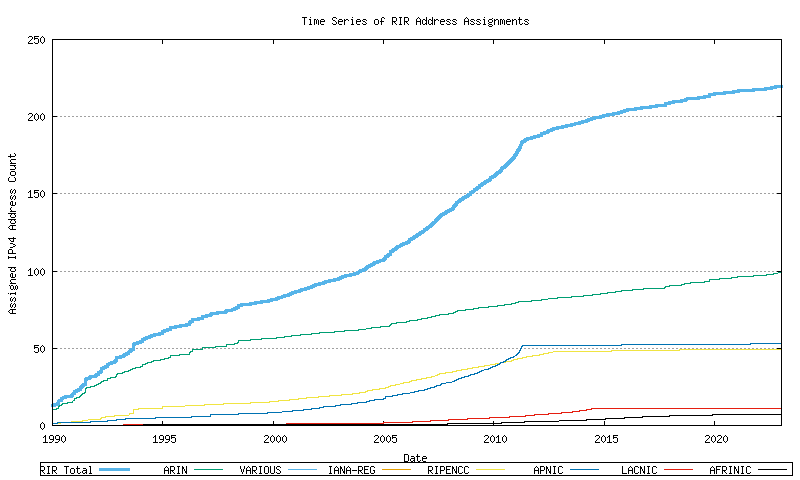
\includegraphics[width=0.8\textwidth]{fig09.png}
  \\
  {\tiny Source: \parencite{IPv4AddressReport}}
\end{frame}

\begin{frame}
\small
\begin{block}{\textit{RFC 1338 — Supernetting: an Address Assignment and Aggregation Strategy}}
\vspace{0.5em}
\textit{It does not attempt to solve the third problem,
which is of a more long-term nature, but instead endeavors to ease
enough of the short to mid-term difficulties to allow the Internet to
continue to function efficiently while progress is made on a longer-
term solution.}
\end{block}
(The third problem being IPv4 exhaustion)
\centering
\\
{\tiny Source: \parencite{fullerSupernettingAddressAssignment1992}}
\end{frame}

\begin{frame}{Timeline of stopgap measures}
\centering
\small
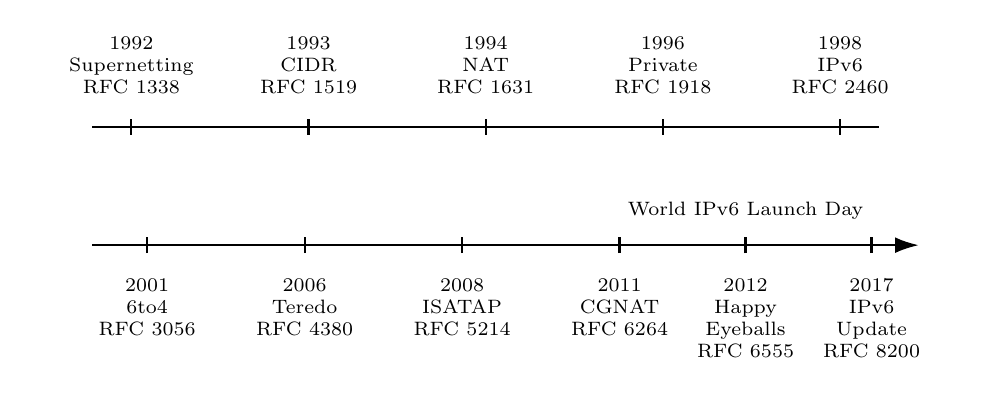
\begin{tikzpicture}[
    x=1cm, y=1cm,
    every node/.style={align=center,font=\scriptsize},
    >=Latex
]
    \def\upperY{0.8}
    \def\lowerY{-0.7}

    \draw[thick] (0, \upperY) -- (10, \upperY);
    \draw[thick, -{Latex[length=3mm,width=2mm]}] (0, \lowerY) -- (10.5, \lowerY)
        node[right, font=\scriptsize, xshift=2mm] {};

    \foreach \xu/\txt in {
        0.5/{1992\\Supernetting\\RFC 1338},
        2.75/{1993\\CIDR\\RFC 1519},
        5.0/{1994\\NAT\\RFC 1631},
        7.25/{1996\\Private\\RFC 1918},
        9.5/{1998\\IPv6\\RFC 2460}
    }{
        \draw[thick] (\xu, \upperY-0.1) -- (\xu, \upperY+0.1);
        \node[above=3mm, text width=2.4cm] at (\xu, \upperY) {\txt};
    }

    \foreach \xl/\txt in {
        0.7/{2001\\6to4\\RFC 3056},
        2.7/{2006\\Teredo\\RFC 4380},
        4.7/{2008\\ISATAP\\RFC 5214},
        6.7/{2011\\CGNAT\\RFC 6264},
        8.3/{2012\\Happy\\Eyeballs\\RFC 6555},
        9.9/{2017\\IPv6\\Update\\RFC 8200}
    }{
        \draw[thick] (\xl, \lowerY-0.1) -- (\xl, \lowerY+0.1);
        \node[below=3mm, text width=2.4cm] at (\xl, \lowerY) {\txt};
    }

    \def\ipv6LaunchX{8.3}
    \draw[thick] (\ipv6LaunchX, \lowerY-0.1) -- (\ipv6LaunchX, \lowerY+0.1);
    \node[above=2mm, text width=3cm] at (\ipv6LaunchX, \lowerY) {World IPv6 Launch Day};
\end{tikzpicture}

\vspace{0.4cm}
\footnotesize
\textit{Timeline of measures from Supernetting to IPv6 'v2'}
\end{frame}


\begin{frame}{IPv6}
  \begin{itemize}
    \item \textbf{RFC 2460} – \emph{Internet Protocol, Version 6}
    \item Finished in 1998 later updated in 2017
    \item Designed to fix the issues of IPv4
    \item Increases the address space from 32-bit to 128-bit
    \item 340 282 366 920 938 463 463 374 607 431 768 211 456 addresses
    \item Allows for some cool things like NAT64
  \end{itemize}
  \centering
  {\tiny Source: \parencite{hindenInternetProtocolVersion1998}, \parencite{deeringInternetProtocolVersion2017}}
\end{frame}

\begin{frame}{Dual-stack}
\small
\begin{block}{\textit{RFC 1933 — Transition Mechanisms for IPv6 Hosts and Routers}}
\vspace{0.5em}
\textit{The most straightforward way for IPv6 nodes to remain compatible with
IPv4-only nodes is by providing a complete IPv4 implementation. IPv6
nodes that provide a complete IPv4 implementation in addition to
their IPv6 implementation are called "IPv6/IPv4 nodes." IPv6/IPv4
nodes have the ability to send and receive both IPv4 and IPv6
packets. They can directly interoperate with IPv4 nodes using IPv4
packets, and also directly interoperate with IPv6 nodes using IPv6
packets.}
\end{block}
\centering
{\tiny Source: \parencite{nordmarkTransitionMechanismsIPv61996}}
\end{frame}

\section{The issue with Dual-Stacking}
\begin{frame}{IPv6 and IPv4 failure rate}
  \centering
  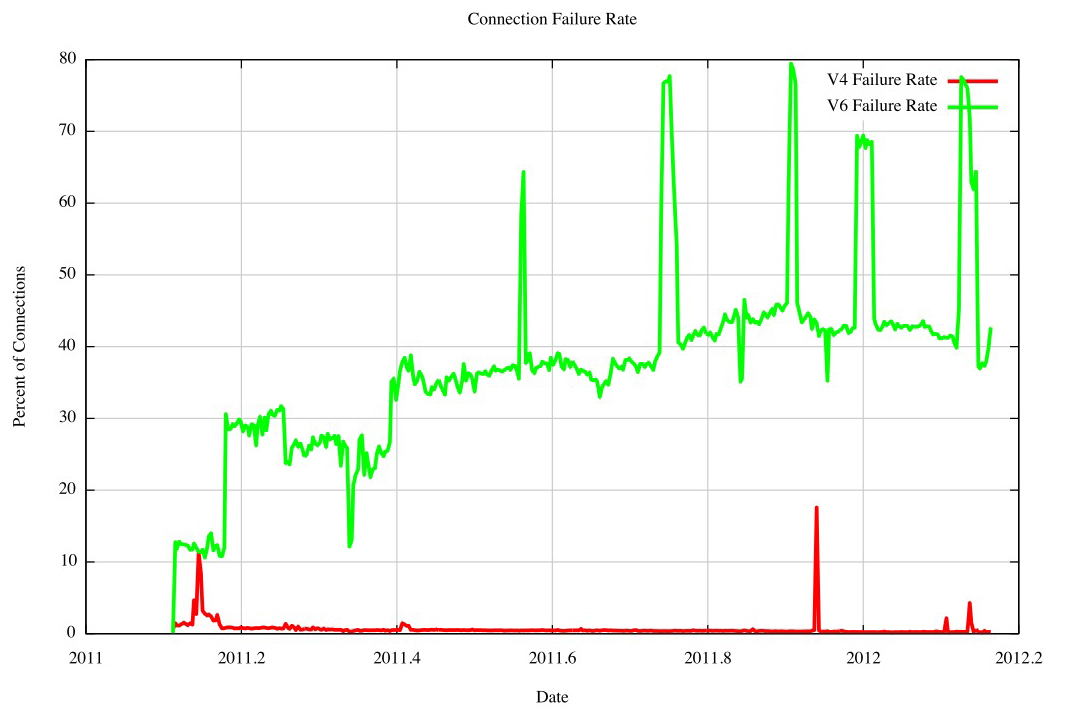
\includegraphics[width=0.7\textwidth]{fig2.jpg}
  \\
  {\tiny Source: \parencite{ISPColumnNovember}}
\end{frame}

\begin{frame}{Dual-Stacking with IPv6 failure}
  \centering
  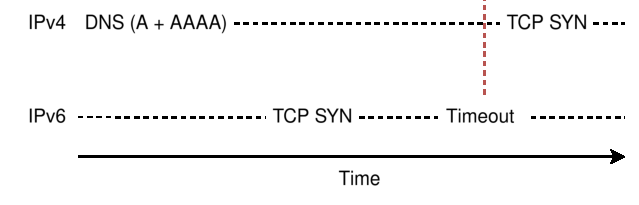
\includegraphics[width=0.9\textwidth]{nohe.pdf}
\end{frame}

\section{The solution}

\begin{frame}{Happy Eyeballs}
  \begin{itemize}
    \item \textbf{RFC 6555} – \emph{Happy Eyeballs: Success with Dual-Stack Hosts}
    \item "Races" IPv4 and IPv6 in order to solve blocking behavior
    \item Applicable to connection oriented transport protocols
    \item Tries to define a set of standard practices around AAAA DNS records
    \item No multi-record AAAA responses within the same namespace
    \item No AAAA specific namespaces e.g. \textit{ipv6.example.com}
    \item Specifies a head start of 150-250 ms but, all browsers use 300 ms
  \end{itemize}
  \centering
  {\tiny Source: \parencite{wingHappyEyeballsSuccess2012}}
\end{frame}

\begin{frame}{Dual-stacking with Happy Eyeballs}
  \centering
  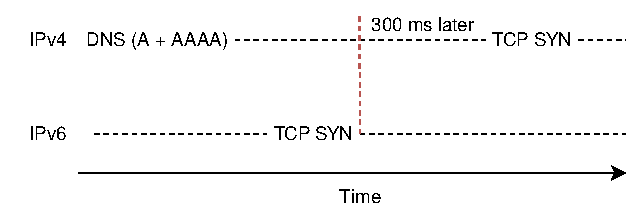
\includegraphics[width=0.9\textwidth]{withhe.pdf}
\end{frame}

\section{Issues with Happy Eyeballs}
\begin{frame}{DNS slow family blocking}
  \centering
  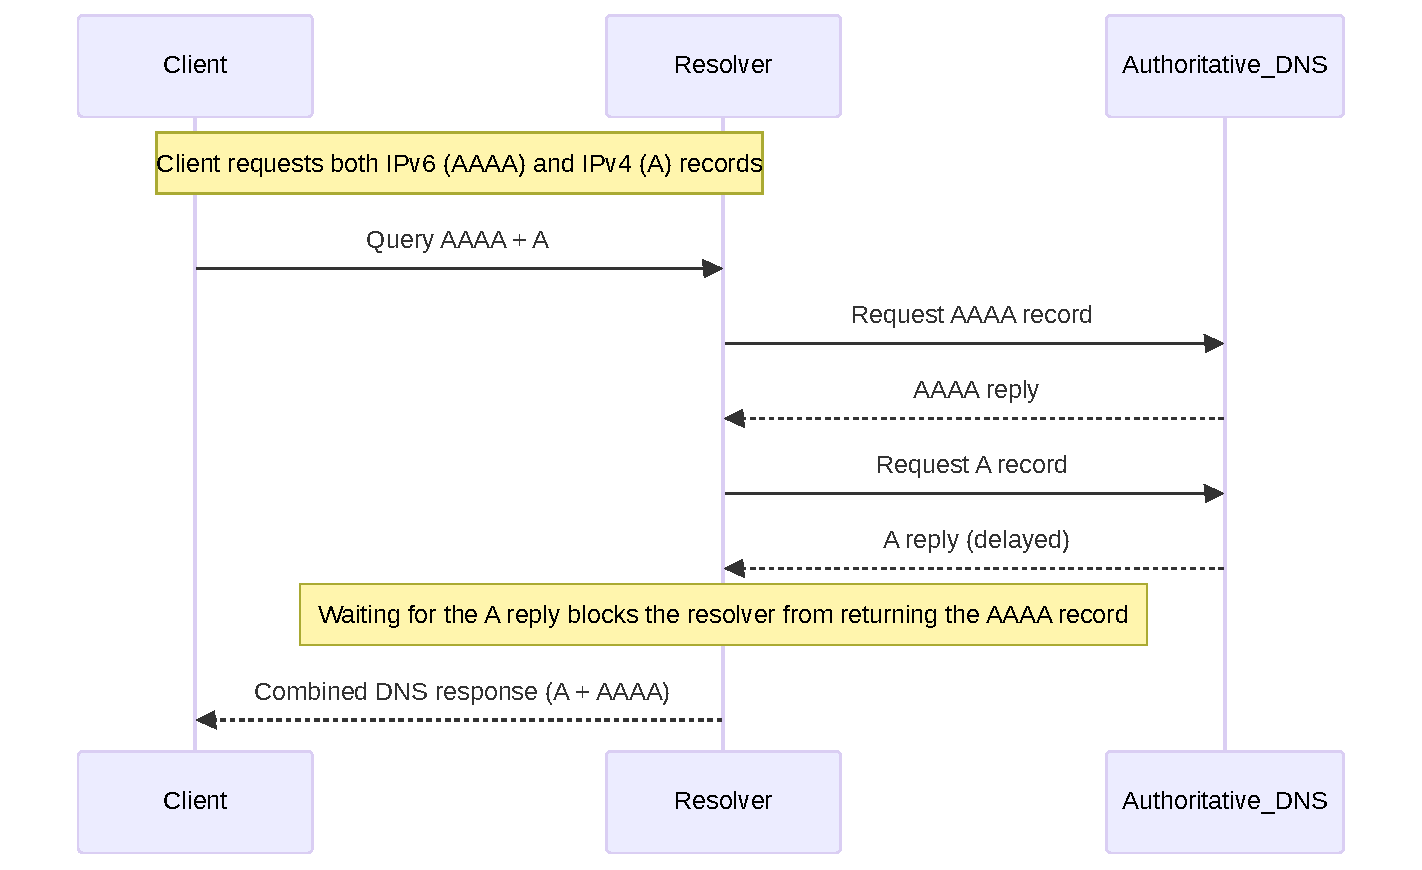
\includegraphics[width=0.8\textwidth]{sfblocking.pdf}
\end{frame}

\begin{frame}{Slower Connections}
\begin{block}{\textit{Measuring the Effects of Happy Eyeballs}}
\vspace{0.5em}
\textit{In 90\% of these cases, HE
tends to prefer slower IPv6 connection. This shows that the timer
value (300 ms) used by the HE algorithm has past its time and is
not suitable in today’s landscape.}
\end{block}
  \centering
  {\tiny Source: \parencite{bajpaiMeasuringEffectsHappy2016}}
\end{frame}

\section{Happy Eyeballs version 2}
\begin{frame}{Happy Eyeballs version 2}
  \begin{itemize}
    \item \textbf{RFC 8305} – \emph{Happy Eyeballs: Better Connectivity Using Concurrency}
    \item Races DNS families to avoid blocking
    \item Races multiple records in multi record DNS responses
    \item Implements a set of 10 rules for sorting the records (Functionally replacing old IPv6 address selection policy defined in \textbf{RFC 3484})
    \item Prefers DNS over IPv6 but, won't race them if both IPv4 and IPv6 addresses are available
    \item Implements a 'resolution delay' to give AAAA records a head start
  \end{itemize}
  \centering
  {\tiny Source: \parencite{schinaziHappyEyeballsVersion2017}}
\end{frame}


\section{Wrap-up}
\begin{frame}
  \centering
  \vfill
  {\usebeamerfont{title}\usebeamercolor[fg]{title}\LARGE Questions?}
  \vfill
\end{frame}

\begin{frame}[allowframebreaks]{References}
  \printbibliography
\end{frame}
\end{document}
